\documentclass[twoside,10pt]{article}

\usepackage{fancyvrb}

% ------
% Fonts and typesetting settings
\usepackage[sc]{mathpazo}
\usepackage[T1]{fontenc}
\linespread{1.05} % Palatino needs more space between lines
\usepackage{microtype}


% ------
% Page layout
\usepackage[hmarginratio=1:1,top=32mm,columnsep=20pt,margin={2.54cm,2.54cm}]{geometry}
\usepackage[font=it]{caption}
\usepackage{paralist}
\usepackage{multicol}

% ------
% Lettrines
\usepackage{lettrine}


% ------
% Abstract
\usepackage{abstract}
	\renewcommand{\abstractnamefont}{\normalfont\bfseries}
	\renewcommand{\abstracttextfont}{\normalfont\small\itshape}

% ------
% Titling (section/subsection)
\usepackage{titlesec}
\renewcommand\thesection{\Roman{section}}
\titleformat{\section}[block]{\large\scshape\centering}{\thesection.}{1em}{}


% ------
% Header/footer
\usepackage{fancyhdr}
	\pagestyle{fancy}
	\fancyhead{}
	\fancyfoot{}
	\fancyhead[C]{Advanced Operating Systems $\bullet$ April 2015}
	\fancyfoot[RO,LE]{\thepage}


% ------
% Clickable URLs (optional)
\usepackage{hyperref}

% ------
% Maketitle metadata
\title{\vspace{-15mm}%
  \fontsize{24pt}{10pt}\selectfont \textbf{Don't Rely On Me:}\\
  \textbf{Evaluating the Applicability of Lock-free Queues in High-Load Web
    Servers} } 
\author{%
  \large
  \textsc{Benjamin Barg $\bullet$ Ruchir Khaitan}\\[2mm]
  \normalsize \href{mailto:bbb2123@columbia.edu}{bbb223@columbia.edu}
    $\bullet$ \href{mailto:rk2660@columbia.edu}{rk2660@columbia.edu}\\
  \normalsize	Columbia University
  \vspace{-5mm} } 
\date{}

% ------
% Including images
\usepackage{graphicx}

% ------
% Using figures inside multicol
\newenvironment{Figure}
  {\par\medskip\noindent\minipage{\linewidth}}
  {\endminipage\par\medskip}

%%%%%%%%%%%%%%%%%%%%%%%%
\begin{document}

\maketitle
\thispagestyle{fancy}

\begin{abstract}
  \noindent Using lock-free queue implementations taken from various
  authors, we present a measurement and comparison study of the
  performance of multithreaded web servers that use these queues to
  perform inter-thread communication for a producer-consumer
  workflow. We then compared our web servers to existing open source
  options \verb+nginx+, \verb+lighttpd+, and \verb+apache+. This
  comparison evaluates the relative performance of a server
  architecture driven by queue message passing versus event polling or
  thread spawning to see how effective lock free queues are for this
  class of program. Results from on an 8 core system show that servers
  built with various lock free queues are significantly more
  performant than ones built with globally locked queues, particularly
  under latency measurements. The lock free servers also outperform
  \verb+apache+ and \verb+lighttpd+ by 
\end{abstract}

\begin{multicols}{2}
  \lettrine[nindent=0em,lines=3]{I}n the past 20 years, there has been
  an explosion of research into lock-free synchronization. Lock-free
  objects possess numerous provable guarantees lacked by locked
  objects, including deadlock immunity and async-signal safety. In
  addition, operations on lock-free data structures have the potential
  to be significantly faster than those on comparable locked objects,
  particuarly under heavy contention. In a world where heavily
  multicore processors are widely available, user-level applications
  are well-behooved to use data structures optimized for the
  distributed nature of multiple cores.
  
High performance web servers provide an intriguing application for
lock-free algorithms, given that they deal with extremely high
concurrency and in certain situations would benefit from progress
guarantees (a good example would be an ad exchange server where each
request represents explicit monetary value). We observe that most
modern servers targeted towards high-concurrency (in particular
\verb+nginx+) have shied away from user-level job distribution and
instead rely on kernel mechanisms for reporting on file descriptors
(the so-called "event-based" server architecture). Our goal is to
explore the limitations of a thread-pooled server architecture that
uses a queue for job distribution through comparison with both a
locked version of the same architecture and with popular modern
high-performance web servers.

\section{Related Work}

The related work for this paper can be split into three sections:
queue implementations, web server architectures, and web
server benchmarking.

\subsection{Blocking locked queues}

The idea of singaling mechanism for locked data structures first
proposed by Hoare in his seminal 1974 paper on monitors
\cite{hoare1974monitors}. As an example within the paper, Hoare
describes the use of condition variables to signal the appearemnce of
new elements in an SPSC queue, and he describes a generalization to
multiple consumers. A standard for conditional variables in which the
signaling threads holds the mutex while signaling was included as an
extension to the POSIX standard in 1992 and was implemented by Mueller
in 1993 \cite{ieee1992pthreads,mueller1993library}.

\subsection{Lock-free queues}

Lock-free programming has been an active area of research for at least
the past thirty years. Michael and Scott present a linked list based
nonblocking queue (referred to as the MS-queue) \cite{MS96}. Their
implementation relies on the compare-and-swap primitive (CAS) that
allows for atomic manipulation of linked list pointers. Kogan and
Petrank give a wait-free variant of the MS-queue \cite{KP11}. However
both these, and other versions of the MS-queue suffer from scalability
problems after a small amount of concurrency because threads contend
for memory locations to perform CAS, and often get stuck in retry
loops that are prohibitively expensive.

Other researchers (Hendler et al, Fatourou and Kallimanis) have shown
that combining-based queues perform better than CAS queues, where a
combining queue essentially serializes access to the queue by only
allowing one thread to perform operations on the queue \cite{He10,
  FK12}. The other threads publish their intended operation on a
shared array. The idea is that past a small amount of threads, CAS
based queue performance degrades so much as to be entirely useless,
and instead sequential access is preferable. In practice, combining
queues have an even greater advantage as the combining thread is
pinned to a single CPU, and stays cache-hot throughout its execution.

Finally, Afek and Morrison present a linearizable concurrent
non-blocking queue based on a linked list of concurrent ring buffers
(LCRQ) \cite{AM13}. This queue avoids the CAS contention problems that
plague MS-queue variants by using theoretically weaker primitives like
fetch-and-add (FA). This queue ends up being significantly faster than
all previous lock-free queues.

\subsection{Web server architectures}

The two most popular (and open-source) servers in current usage are
\verb+apache+ and \verb+nginx+, and each is the prime exponent of a
particular philosophy for web server architecture. \verb+apache+
follows the fork-on-request model, where each connection is assigned a
separate process that fulfills the requests and them terminatoes
\cite{fielding1997apache}. \verb+nginx+ uses an ``event-based''
architecture, where a fixed number of worker threads poll a set of
file descriptors \cite{syosevnginx}. This approach relies on the
existence of fast kernel polling mechanisms: \verb+epoll+ for Linux
and \verb+kqueue+ for BSD-based systems. \verb+lighttpd+ is another
minimal web server using at event-based architecture
\cite{kneschke2003lighttpd}.

Existing event-based servers have demonstrated reasonably better
performance than thread-per-request servers. In a comparative study
between finely tuned event-based and thread-per-request servers
(optimized by the researchers themselves) Pariag et al. demonstrated
an 18\% throughput advantage for the event-based server
\cite{pariag2007comparing}.

\subsection{Server performance testing}

Conducting meaningful benchmarks of web server performance is
challenging because web servers have many potential bottlenecks,
including but not limited to the file system cache, network
variability and efficiency of multithreading or multiprocessing.

Multiple open-source applications exist for conducting benchmarks for
the serving of static content. Apache bench (\verb+ab+) and
\verb+lighttpd+'s \verb+weighttpd+ both allow the user to specify the
number of connections, connection rate, number of client threads, and
concurrency level
\cite{fielding1997apache,kneschke2003lighttpd}. \verb+nginx+'s
\verb+wrk+ provides a similar interface, but focuses on maintaining a
certain number of concurrent connections. \cite{syosevnginx}. HP's
\verb+httperf+ includes all of the former functionality and adds more
extensive data reporting \cite{mosberger1998httperf}.

Benchmarking performance while scaling number of cores presents a
particular challenge, with researchers aggressively tuning benchmarks
to isolate particular elements of the web server stack. Hashemian
describes strategies for benchmarking servers on multicore systems,
with workloads that attempt to isolate the performance of the TCP/IP
stack and of application-level activity respectively
\cite{hashemian2013improving}. Veal and Foong present a detailed
analysis of the performance scalability of multicore web servers, from
which they concludue that the primary bottlenecks inhibiting web
server scalability were system bus hardware design flaws
\cite{veal2007performance}. Geneves shows that bus saturation
continues to be an issue as recently as 2012
\cite{geneves2012analysis}.

\section{Implementation}

We test three implementations of thread-pooled, queue-based web
servers, which we refer to from here on as \verb+locked-server+,
\verb+msq-server+, and \verb+lcrq-server+. These implementations serve
static content on a single port, with worker threads sleeping if the
work queue is empty. A single acceptor thread loops on accept and adds
connections to the queue (in the form of client socket file
descriptors) as they arrive. All three servers are written solely in C
and use the POSIX sockets library directly to create and serve client
sockets. By default, the servers support logging of incoming
connections to \verb+stdout+, although in Section 4 we observe a
marked performance increase when logging is disabled.

It should be clarified that none of \verb+locked-server+,
\verb+msq-server+, or \verb+lcrq-server+ are intended as full-featured
and robust servers that would at this point in time be used to replace
existing servers (although the their feature-set is not extremely far
away from that of \verb+lighttpd+). Our goal is to compare
event-based, queue-based, and fork-on-request server architectures
under extremely high load, so we have chosen minimal queue-based
implementation to isolate the performance of the queue within the
server.

Also, we must stress that the servers as a whole are emphatically not
lock-free. They use lock-free queues for inter thread communication,
but everything else such writing logs to disk, accessing files, or
allocating memory is done with standard library functions and system
calls. While the progress guarantees of lock free algorithms are
valuable, this paper is more concerned with the potential performance
benefits from using lock-free data structures as part of a
not necessarily lock-free application.

We implemented web servers using three different parallel queue
algorithms, as detailed below.

\subsection{\texttt{locked-server}}

This version of the server is the basis for the others, and uses a
singly-locked queue (one lock is used for both enqueueing and
dequeueing). The queue also uses a POSIX condition variable to synchronize
access so that worker threads don't have to poll the queue and instead may
sleep on when no jobs are available.

\subsection{\texttt{msq-server}}

This version is a modified copy of \verb+locked-server+ with the single
locking queue replaced by an implementation of Michael and Scott's
seminal MPMC lock-free queue \cite{synch-1.0.1}. POSIX
condition variables can no longer be used to implement sleeping on an
empty queue; instead we use a light wrapper over the \verb+futex+ system
call. This particular implementation of the Michael and Scott queue
returns -1 whenever a \verb+dequeue+ fails on an empty queue. 

\subsection{\texttt{lcrq-server}}

Also a modified copy of \verb+http-sever+, \verb+lcrq-server+ replaces
the locking queue with an implementation of Morrisson and Afek's
so-called LCRQ \cite{lcrq-source}. The LCRQ is a linked list of ring buffers that uses
fetch-and-add as its primary atomic primitive (when performing
operations on an inidividual ring buffer), falling back to
compare-and-swap only when the new ring buffers need to be added to
the linked list. Although LCRQ is an MPMC queue, we only have a single
accepting thread and thus a single enqueuer. Like for the Michael
Scott queue, \verb+dequeue+ returns -1 on an empty queue. 

\subsection{Queue optimizations}

We could not use POSIX condition variables with the lock free queues
because condition variables are bound to a specific lock, and that
would be identical to the locked queue. However, our initial
implementations relied on worker threads polling the queues and
spinning on failed dequeues. While this approach worked, it was very
inefficient. 
\verb+counter+.
\begin{Verbatim}[numbers=left,
                 fontsize=\small]
#define MAX_WAKEUP 64

//If addr == old_val, calling thread
//is put on a wait queue until wakeup
int futex_cond_wait(int* addr, int old_val) {
    return syscall(SYS_futex, addr, 
                FUTEX_WAIT_PRIVATE, 
                old_val, NULL, NULL, 0); 
}
//Wakeup n threads listening on addr
int futex_wake(int* addr, int n) {
    if (n > 0) {
        return syscall(SYS_futex, addr, 
        FUTEX_WAKE_PRIVATE, 
        n, NULL, NULL, 0); 
    }
    return -1;
}
int futex_signal(int* addr) {
    return futex_wake(addr, 1); 
}
int futex_broadcast(int* addr) {
    return futex_wake(addr, MAX_WAKEUP); 
}
\end{Verbatim}

First, we optimized this naive approach by using a thin
wrapper over the \verb+futex+ system call to allow the worker threads
to sleep when the queue is empty. Then the acceptor thread woke the
workers whenever it enqueued a new connection.  We also implemented
two different types of wakeups, \verb+signal+ to wake only one
sleeping thread, and \verb+broadcast+ to wake up all sleeping threads.
This intentionally matches POSIX condition variables, and we compare
the performance implications of the two. 

The second optimization uses
an atomic integer to store the number of items in the queue, where
enqueuers increment, and dequeuers decrement on success. This let us
cut down both the number of calls to a \verb+futex+ wakeup function,
as the accepting thread only has to wakeup threads when the queue
transitions from empty to nonempty (the integer increases from zero to
one). Furthermore, this allows dequeuers to determine whether they can
sleep by checking the length of the queue, instead of polling on the
dequeue operation. Both of these optimizations were used in the
\verb+msq-server+ and the \verb+lcrq-server+. 

Since these optimizations don't really modify the semantics of \verb+enqueue+
at all, the function \verb+queue_put+ requires little modification over 
the \verb+enqueue+ operation as defined for the lock free queues. Here, \verb+enqueue+ is guaranteed to always succeed, and then we atomically increment the queue length, which is stored in \verb+futex_addr+, signalling worker threads if the queue was originally empty.   
\begin{Verbatim}[numbers=left,
                 fontsize=\small]
void queue_put(struct queue *q, 
    int* futex_addr, int sock) {
    enqueue(q, sock); 	
    //If queue was empty, wakeup workers 
    if (!(__sync_fetch_and_add(futex_addr, 1))) {
    #ifdef WAKEUP_BROADCAST
        futex_broadcast(futex_addr); 
    #else 
        futex_signal(futex_addr); 
    #endif 
    }
}
\end{Verbatim}

\verb+queue_get+ is slightly more complicated. Here, \verb+dequeue+
comes from the lock-free queue implementations and therefore returns -1 if the
queue is empty. We use \verb+futex_addr+ as before to represent the length of the queue, and we use a\verb+while()+ loop
because the \verb+futex+ system call automatically checks whether the
queue is empty (i.e.  \verb+counter == 0+) before sleeping. We need to
wrap \verb+futex_cond_wait+ with a loop anyways to avoid spurious dequeues.


\begin{Verbatim}[numbers=left,
                 fontsize=\small]
int queue_get(struct queue *q, int* futex_addr) {
    int ret;
    //Check if queue empty or dequeue fails
    //if so sleep  
    while (*futex_addr == 0 || 
        (ret = dequeue(q)) == -1){
        futex_cond_wait(futex_addr, 0);
    }
    //successful deque - now decrement and get out 
    __sync_fetch_and_sub(futex_addr, 1);
    return ret; 
}
\end{Verbatim}

\section{Testing strategy}

Our testing strategy centers around two main goals:

\begin{compactitem}
\item What are the traditional bottlenecks of a queue-based web server
  architecture and how could a lock-free queue possibly circumvent
  those?
\item How closely can an optimized version of a lock-free-queue based
  webserver approach the performance (under heavy load) of existing
  web servers \verb+nginx+, \verb+lighttpd+, and \verb+apache+?
\end{compactitem}

For testing, we make heavy use of HP's \verb+httperf+ utility, which
allows sending adjusting the per-second requests rate and setting
timeouts, and which has the crucial feature of continuing to send
requests without recieving replies from the server
\cite{mosberger1998httperf}. This tool, combined with a fast
enough connection to the server, allows us to max out our servers'
capacity for concurrency.

Our tests were run between two identical rack servers housed in the
same building. Each server has two quad-core Intel Xeon L5420 2.50 GHz
processors, each of which have with a 12 MB L2 cache. Both servers
have 16 GB of RAM, both run Ubuntu 14.04.2 LTS (Linux kernel version
3.13.0-46-generic), and both have a 1TB HP Proliant HardDrive for
storage.

It should be noted that while \verb+nginx+, \verb+lighttpd+,
\verb+apache+ and our servers all send differently-size response
headers, we chose not to normalize filesize to compensate. Our servers
send a header of \verb+18b+, while \verb+nginx+, \verb+lighttpd+, and
\verb+apache+ send headers on the order of \verb+200b+.

\subsection{System tuning}

In all tests run with \verb+httperf+ we use the \verb+--hog+ option,
which ensures that the \verb+httperf+ uses the fully available
ephemeral port range. This option is particularly necessary for
long-running tests with repeated requests for small files, as the
default available port range can become quickly exhausted. Beacuse our
tests were always run with a single client IP, we ran into issues with
repeated test iterations, in which the majority of available ports
would linger in the \verb+TIME_WAIT+ state. These lingering ports
would cause uncharacteristically bad performance on the latency and
throughput workloads. To maintain port availability over multiple
subsequent test, we set \verb+net.ipv4.tcp_fin_timeout+ to one second
and set both \verb+net.ipv4.tcp_tw_recycle+ and
\verb+net.ipv4.tcp_tw_reuse+ to 0.

\subsection{Server latency}

\begin{Figure}
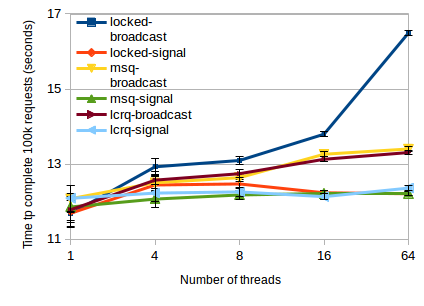
\includegraphics[width=\linewidth]{img/latencynthreads2.png}
\captionof{figure}{Latency test results using signal and broadcast
  semantics, versus number of worker threads}
\end{Figure}
\begin{Figure}
  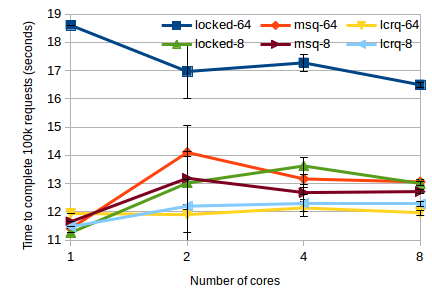
\includegraphics[width=\linewidth]{img/latencyncores.png}
  \captionof{figure}{Latency versus number of cores at with selected
    numbers of worker threads}
\end{Figure}
\begin{Figure}
  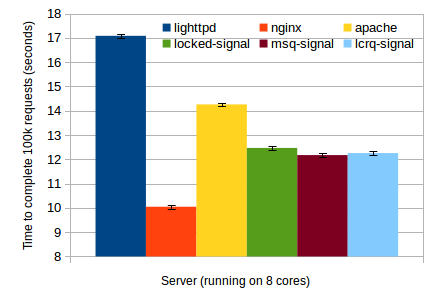
\includegraphics[width=\linewidth]{img/commodityserverlatencies.png}
  \captionof{figure}{When number of worker threads equals number of
    hardware threads, our servers outperform \texttt{apache} and \texttt{lighttpd} on
    the latency workload but are slower than \texttt{nginx}}
\end{Figure}
\begin{Figure}
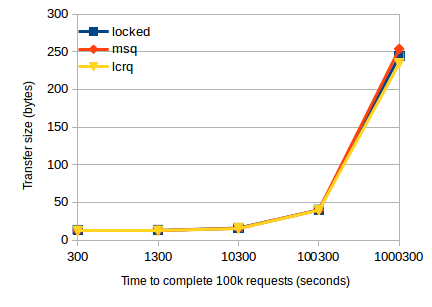
\includegraphics[width=\linewidth]{img/latencyfilesize.png}
\captionof{figure}{All of our servers experience a significant latency
  spike for files around 100Kb, likely due to network saturation}
\end{Figure}

This is a really simple experiment designed to test the server request
latency. We use \verb+httperf+ to send increasing numbers of requests
as fast as possible, and measured the total time required to process
those requests. Larger numbers of files generate longer running test
times, but this gives a better measurement of average processing rate
(requests/second) that takes into account nondeterministic factors
like TCP/IP warmup, network noise, filesystem caching and other factors.

The latency performance of each of these servers varies drastically
based on the thread wakeup policy used. Specifically, do they
\verb+futex-signal+ and only wake up only one available thread, or do
they \verb+futex-broadcast+ and attempt to wakeup as many threads as
possible. Since the latency test workload is inherently serial, ideal
performance should be constant regardless of the number of threads or
cores available, since only one network request ever needs to be
processed at a time. Employing \verb+futex-signal+ allows all three
servers to approach the ideal performance. Unsurprisingly, using
\verb+futex-broadcast+ signficantly degrades server performance,
particularly that of \verb+locked-server+. This is exactly as expected
as increased lock contention is more expensive than increased CAS
retry contention in the MS-queue or increased FAA contention in the
LCRQ.

\subsubsection{Explanation of comparative performance of commodity
  servers}

\verb+nginx+ completes the latency workload roughly 16\% faster than
our queued servers. With filesize, network latency, physical machine
characteristics, and OS tuning controlled for, we find it reasonable
that \verb+nginx+'s main performance benefit comes from its use of
\verb+epoll+ to distributed open connections to workers. For clarity,
our system is defined as the combination of a lock-free SPMC queue and

% - why is nginx faster: translates to why is epoll faster?
% - 

\subsection{Server throughput}

\begin{Figure}
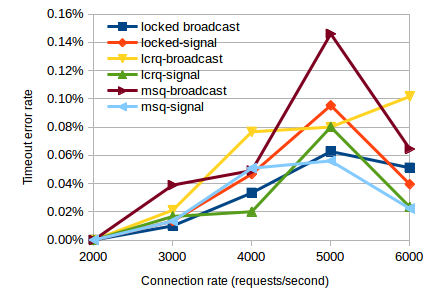
\includegraphics[width=\linewidth]{img/throughputmedian.png}
\captionof{figure}{Throughput data is noisy when comparing signal and
  broadcast semantics. The lock-free servers perform better with
  signal, but the locked server favors broadcast.}
\end{Figure}

Here, requests are sent from a client program at incrementally
increasing rates, and all the requests have a specified
timeout. The maximum rate that the server can respond completely to
with no dropped or refused requests is the server throughput. This
also is a good test of the maximum concurrency the server can support.

We tested our servers at rates ranging from 200 to 6000 requests per
second, always with .1 second timeouts. We chose such a low timeout
because anything much larger than that is so large that all requests
are always satisfied. With httperf, we could not reliably generate
more than 6000 requests per second because httperf relies on the
\verb+select+ system call, which is limited to multiplexing only 1024
file descriptors at a time. This means that if we attempt to generate
higher loads, \verb+httperf+ runs out of file descriptors and the
entire test becomes invalid.

Unfortunately, the restrictive parameters of this test make it very noisy, 
and its hard to draw any conclusions from these results. 

\section{Future work}

To this point, our lock-free server implementations have been done
rather naively. We propose several possible performance optimizations
to push the performance of \verb+msq-server+ and \verb+lcrq-server+
closer to that of \verb+nginx+ and \verb+lighttpd+. In certain cases,
such as application-level content caching, these are optimizations
that already exist in the aforementioned applications.

\subsection{Application level content-cache}
While the OS maintains a file buffer cache, using it requires the
syscall overhead from \verb+read+. To reduce this overhead, several
existing servers (including \verb+nginx+) optionally maintain a
user-level file cache so that more content can be served via
user-space memory access. We have not yet implemented a full cache
solution, but we did simulate the effects of such a cache by modifying
\verb+lcrq-server+ to send static global buffer instead of pulling the
requested file system. This preliminary test also demonstrated a 10\%
performance improvement. We thus expect a fully-featured user-space
content cache to contribute a meaningful speedup.

\subsection{Robust lock-free memory management}

Currently, we do not have a robust lock-free memory allocation or
memory reclamation strategy in place for \verb+msq-server+ and
\verb+lcrq-server+. When new nodes are needed, the acceptor thread
simply calls \verb+malloc+ within each queue implementation to create
a new node. While this reliance on a locking \verb+malloc+ admittedly
affects the supposed progress guarantee of the lock-free algorithms we
use, we hold that it should not signicantly effect performance, as
only the accepting thread is contending for the \verb+malloc+
lock. Usage or implementation of a lock-free (or otherwise robust)
memory allocator would likely \emph{improve} server performance, given the
options for per-thread pooling and CPU memory locality
\cite{hart2007performance}.

As for memory reclamation, the standard and popular lock-free solution
is Maged M. Michael's hazard pointers \cite{michael2004hazard}. Hazard
pointers allow threads operating on a shared lock-free object to
temporarily ensure that hazardous references (for example a pointer to
the next item in a queue) will remain valid as long as the thread
holds one of a finite number of hazard pointers to the object. There
is a small amount of overhead associated with hazard pointers, as the
implementation requires both declaring the lifetime of hazardous
reference within operations on the object and a periodic scanning of
the global list of hazard pointers to lazily free nodes. We
acknowledge that performance for \verb+lcrq-server+ and
\verb+msq-server+ would likely be slower with a hazard pointer
implementation, but we view generating research claims via server
profiling as a higher priority in our current research than the
production of a hazard pointers implementation.

\subsection{Creating a fully lock-free application}

Both \verb+msq-server+ and \verb+lcrq-server+ incorporate a lock-free
queue, but each relies on mutiple locked subsystems, both in the C
standard library and in the Linux kernel (e.g. the sockets library,
\verb+malloc+, the \verb+futex+ system call, and the in-kernel TCP/IP
stack). While some of these systems have user-space solutions\---there
exist, for example, lock-free memory allocators\---others require the
existence of lock-free kernel implementations (in particular, the
\verb+futex+ system call). Further work on lock-free versions of these
systems may follow two possible paths:
\begin{enumerate}
\item implementing lock-free alternatives on a case-by-case basis,
  with the goal of reducing web server bottlenecks 
\item creating a fully lock-free kernel, which aims to provide a
  provably lock-free system
\end{enumerate}

The first of these approaches is probably more relevant to web-server
optimization. A recent patch to the Linux kernel \verb+epoll+ file
descriptor notification system noticed a significant in scalability
when removing lock on the \verb+epoll+ algorithm's fast path
\cite{lockfree-epoll}. Similar optimizations may be possible for the
\verb+futex+ system call.

Implementation have been attempted for lock-free kernels that support
scalability for higher numbers of threads \cite{massalin1992lock}, but
its authors admit that similar performance can be achieved with
user-level thread libraries. A fully-lock free system would be most
beneficial for applications that absolutely require high levels of
thread contention; given the sucess of event-based architectures, web
servers do not appear to fit this model.

\subsection{Lock-free application server}

When serving static files with our queued servers, the only
significant user-space concurrency bottleneck is the distribution of
open connections from the accepting thread to worker threads. However,
modern web servers also serve dynamic content, in which there may be
more instances of high-contention data structures.

Database servers seem to be a particular fruitful ground for lock-free
applications, since they must support high numbers of concurrent
operations. Hekaton, a database engine included in the 2014 version of
Microsoft's SQL server, uses a lock-free fast path for designated
in-memory tables to support large numbers of concurrent operations
\cite{diaconu2013hekaton}.

Web servers using pipeline parallelism, in which a stages of a
sequential workflow are parallelized and then synchronized at various
steps, present another application for lock-free queues in web
servers. Giacomoni et al. showed that a lock-free queue with heavy
cache-locality optimization can provide significant performance
benefits on a network frame processing workflow
\cite{giacomoni2008fastforward}.

\section{Conclusion}

We have implemented a set of HTTP/1.0 web servers that serve static
content and that rely on a lock-free SPMC queue to distribute active
connections to worker threads. In adapting normally non-blocking
algorithms to a blocking-wait context, we implemented a simple
condition variable system with the Linux \verb+futex+ system call and
an atomically modified integer which keeps track of the size of the
queue. Our benchmarks of these servers show a clear latency advantage
for both the LCRQ and MSQ lock-free queues over a locked variant, as
well over both fork-on-request-based and event-based commodity
servers. While throughput tests do not exhibit a clear advantage for
the lock-free servers, these tests do demonstrate that the lock-free
servers perform similary to \verb+lighttpd+ and \verb+apache+.

However, our tests show that the event-based server \verb+nginx+ holds
a clear performance advantage over our lock-free servers. We attribute
\verb+nginx+'s advantage to its use of the \verb+epoll+
event-notification system, which incurs less system call overhead and
eliminates spurious wakeup. Given the success of \verb+nginx+, it
appears that any possible further benefit from incorporating lock-free
data structres into event-notification systems will come at the kernel
level and not in user space.

% For the remainder of our project, we consider the following to be our
% main deliverables:

% \begin{compactitem}
% \item A comprehensive test bench available as a git repository that
%   can be used to replicate our tests
% \item Results from a large number of iterations of our test bench,
%   with the goal of decididing on meaningful error bounds for
%   performance measurements
% \item A heavily-optimized version of \verb+lcrq-server+, utilizing the
%   optimization techniques suggested in Section IV
% \item Itemized conclusions explaining \emph{why} \verb+lcrq-server+
%   performs better or worse on specified tests.
% \end{compactitem}

\end{multicols}

{\small
  \bibliographystyle{abbrv}
  \bibliography{ref}
}

\end{document}
